\chapter{SAF microarchitecture conceptual framework}
\label{chapter:conceptual_framework}

\section{Sparse smartbuffer model}

\subsection{Composition}

\begin{figure}[ht]
    \centering
    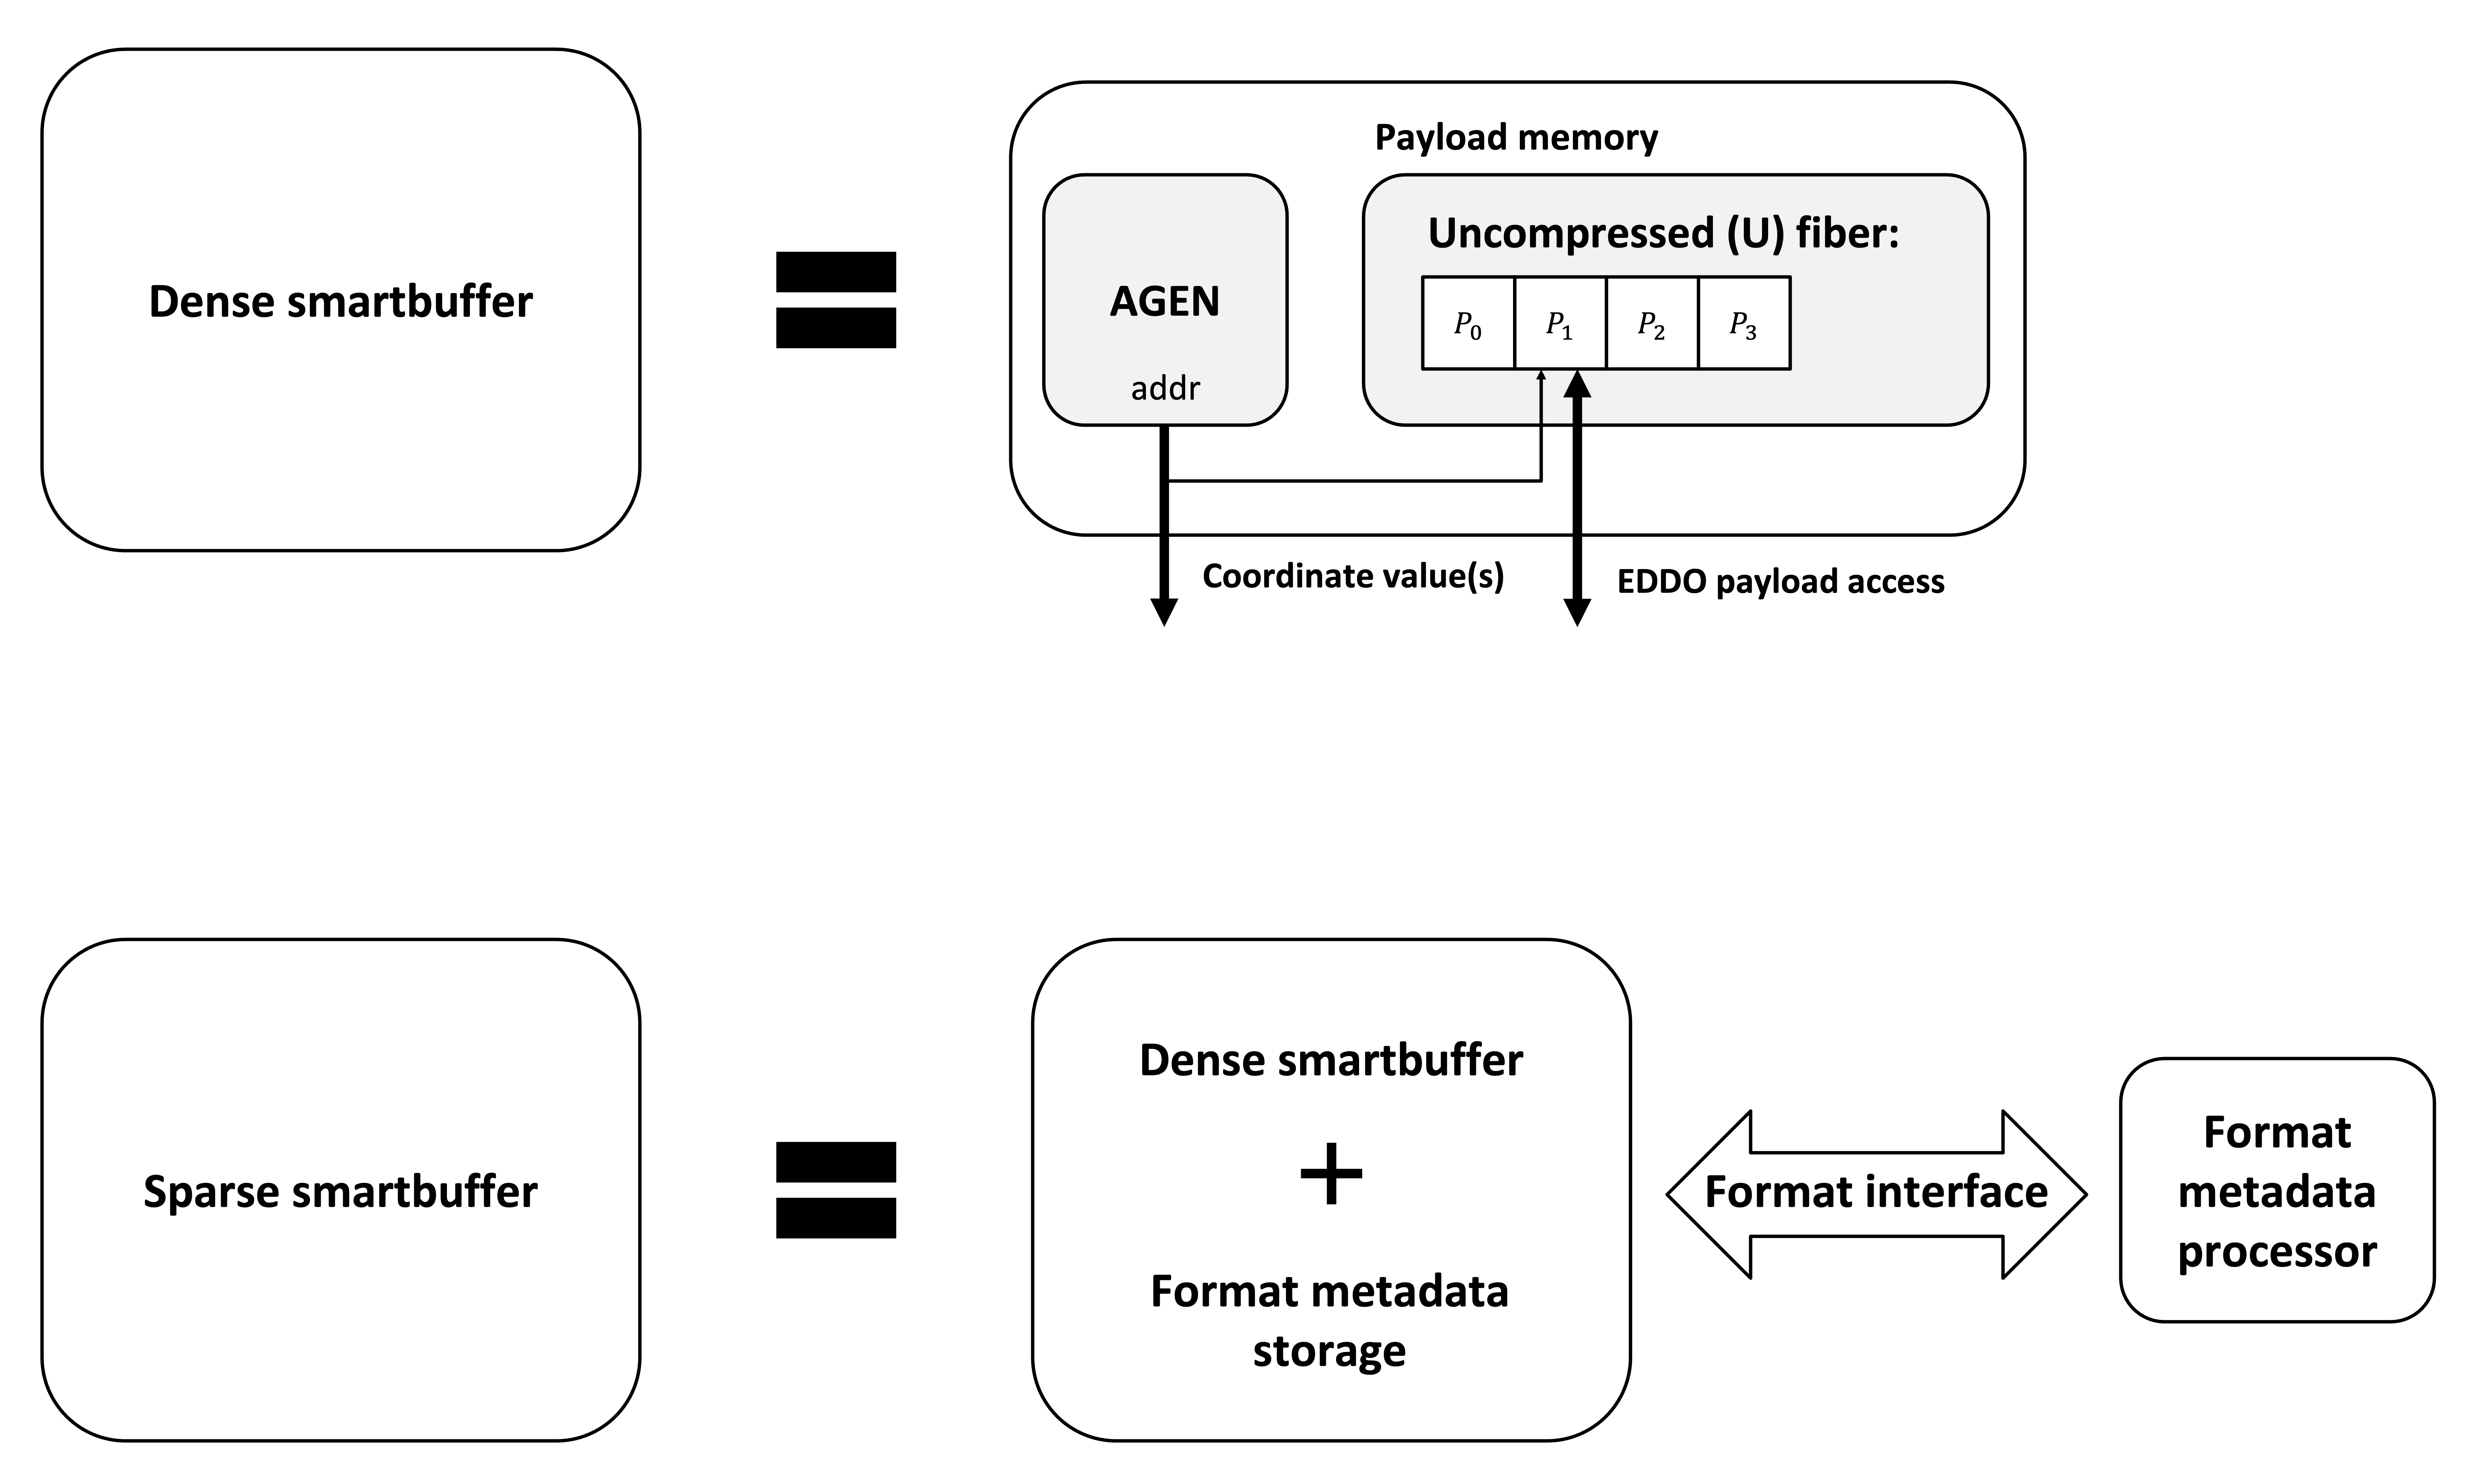
\includegraphics[width=0.95\textwidth]{figures/dense_smartbuffer_composition.png}
    \caption{This work models a \textit{sparse smartbuffer} as the composition of a dense smartbuffer with additional hardware that handles the compressed sparse tensor format, connected by an I/O bundle (``format interface''.) The format interface moves sparse format metadata from the dense smartbuffer metadata storage to the format metadata processor, and moves control signals in the other direction.}
    \label{fig:dense_smartbuffer_composition}
\end{figure}

\subsection{Single-rank, explicit-coordinate-format sparse smartbuffer model}

\begin{figure}[ht]
    \centering
    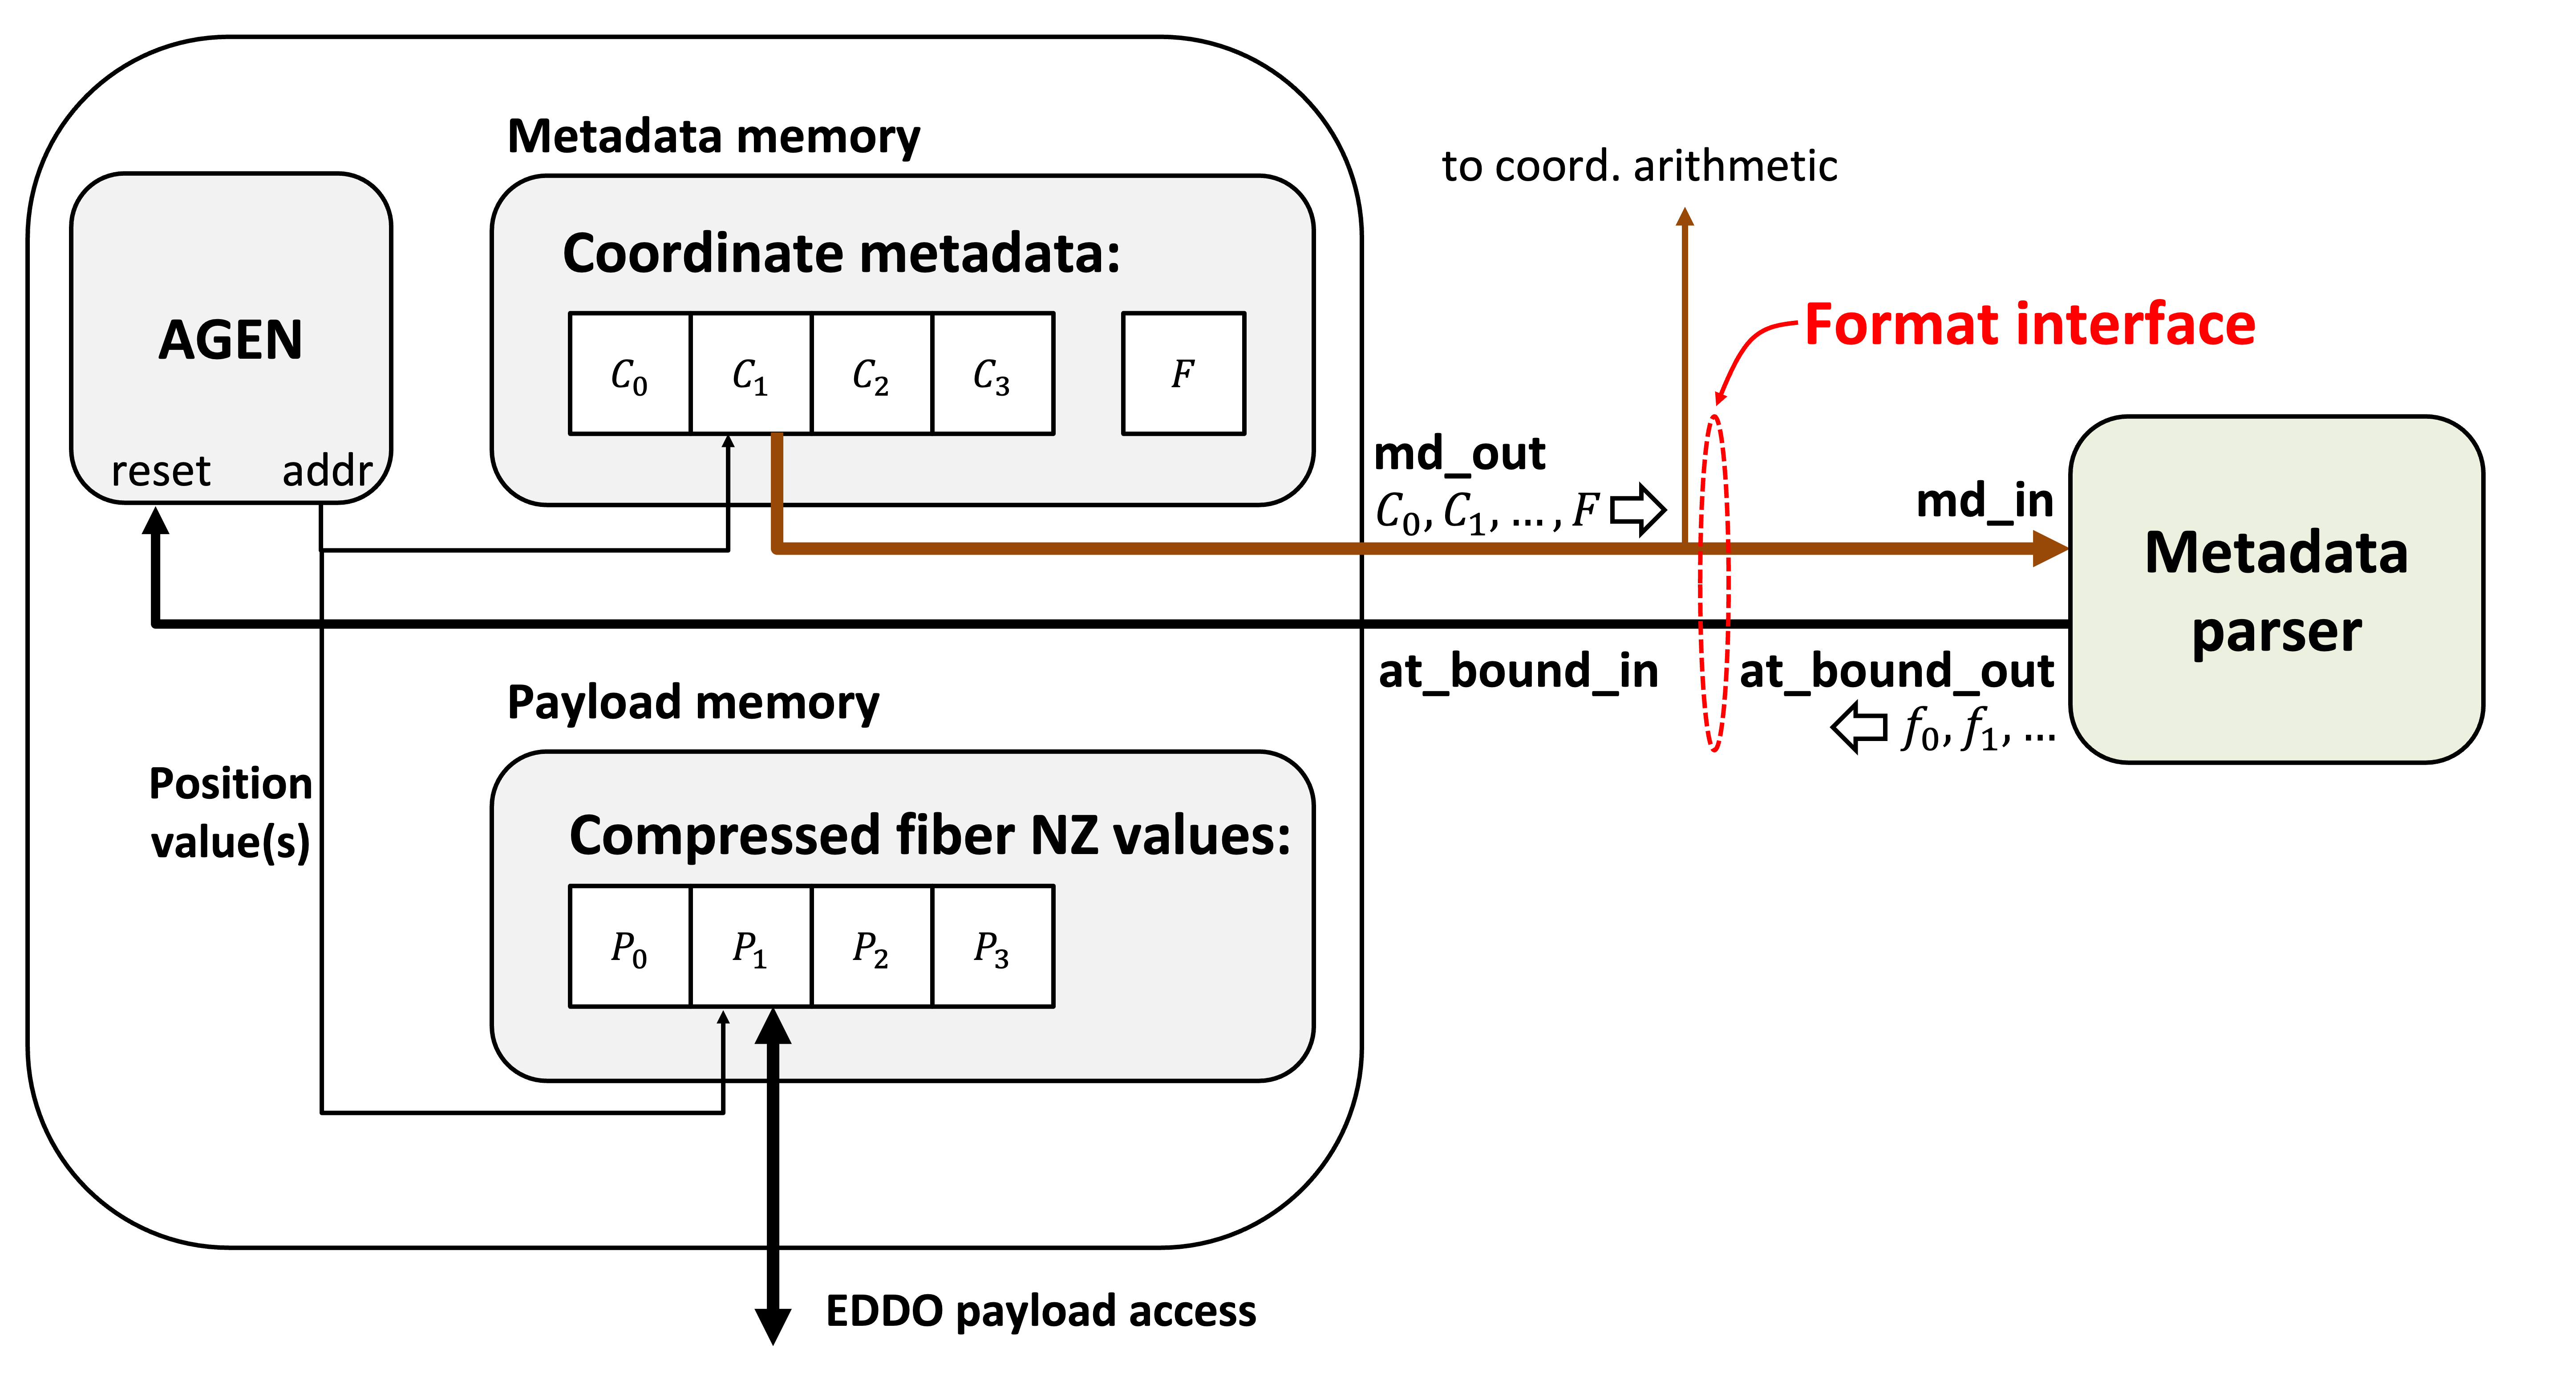
\includegraphics[width=0.95\textwidth]{figures/single_rank_explicit_coordinate_smartbuffer_model.png}
    \caption{Sparse smartbuffer model for a single rank, supporting explicit coordinate sparse tensor formats. ${C_i}$ are explicit coordinate metadata values. $F$ is a stand-in for any metadata regarding fiber characteristics, i.e. number-of-non-zeros. ${f_i}$ are flag values - metadata parser parses metadata arriving at md\_in and sets at\_bound\_out when fiber traversal is complete.}
    \label{fig:single_rank_explicit_coordinate_smartbuffer_model}
\end{figure}

\subsection{Single-rank, general-format sparse smartbuffer model}

\begin{figure}[ht]
    \centering
    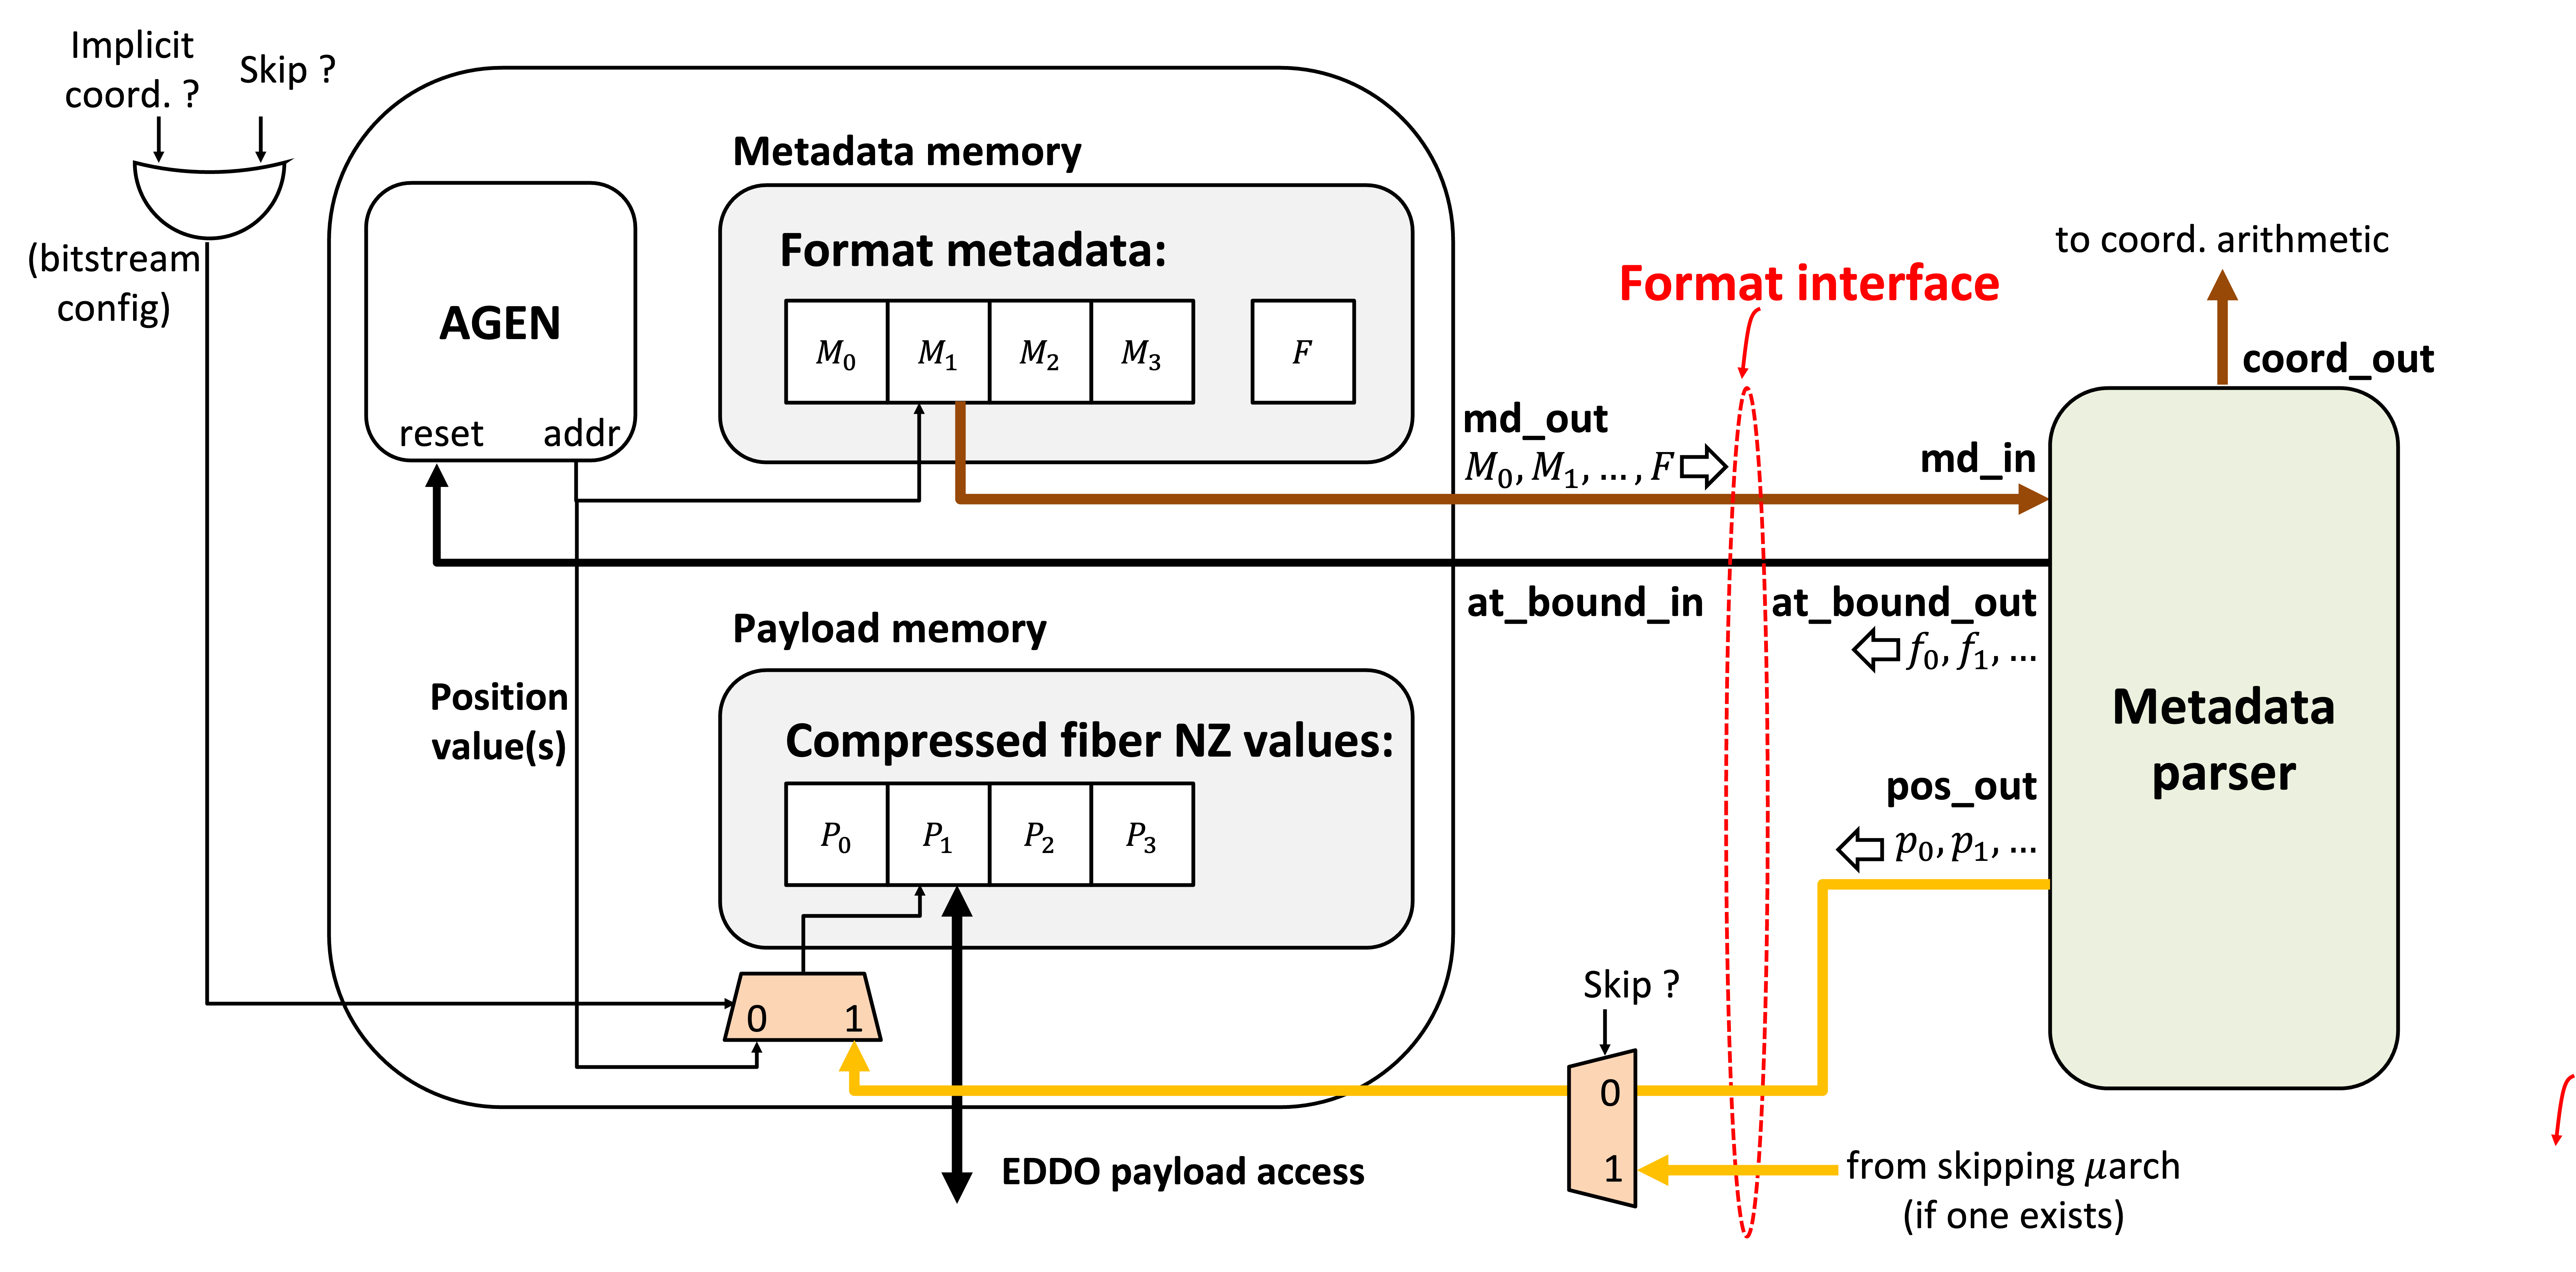
\includegraphics[width=0.95\textwidth]{figures/single_rank_general_format_smartbuffer_model.png}
    \caption{Sparse smartbuffer model for a single rank, supporting general sparse tensor formats. ${M_i}$ are general sparse metadata values, which may not be explicit coordinates. The metadata parser can orchestrate payload reads (via pos\_out) if this is enabled in the configuration bitstream. This is necessary for implicit coordinate representation formats. If skipping is enabled in the configuration bitstream, a skipping microarchitecture's output position stream can orchestrate payload reads. The functionality of the at\_bound\_out signal is unchanged. }
    \label{fig:single_rank_general_format_smartbuffer_model}
\end{figure}

\subsection{Multi-rank-pipelined (hierarchical), general-format sparse smartbuffer model}

\begin{figure}[ht]
    \centering
    \includegraphics[width=0.95\textwidth]{figures/hierarchical_general_format_sparse_smartbuffer.png}
    \caption{A sparse smartbuffer that stores a multi-rank tensor, inspired by the ExTensor\cite{extensor} design for traversing and intersecting deep fibertrees. The format microarchitecture implements a rank-parallel metadata processing pipeline. See Figure~\ref{fig:format_interface} for the structure of the format interface I/O bundle.}
    \label{fig:hierarchical_general_format_sparse_smartbuffer}
\end{figure}

\begin{figure}[ht]
    \centering
    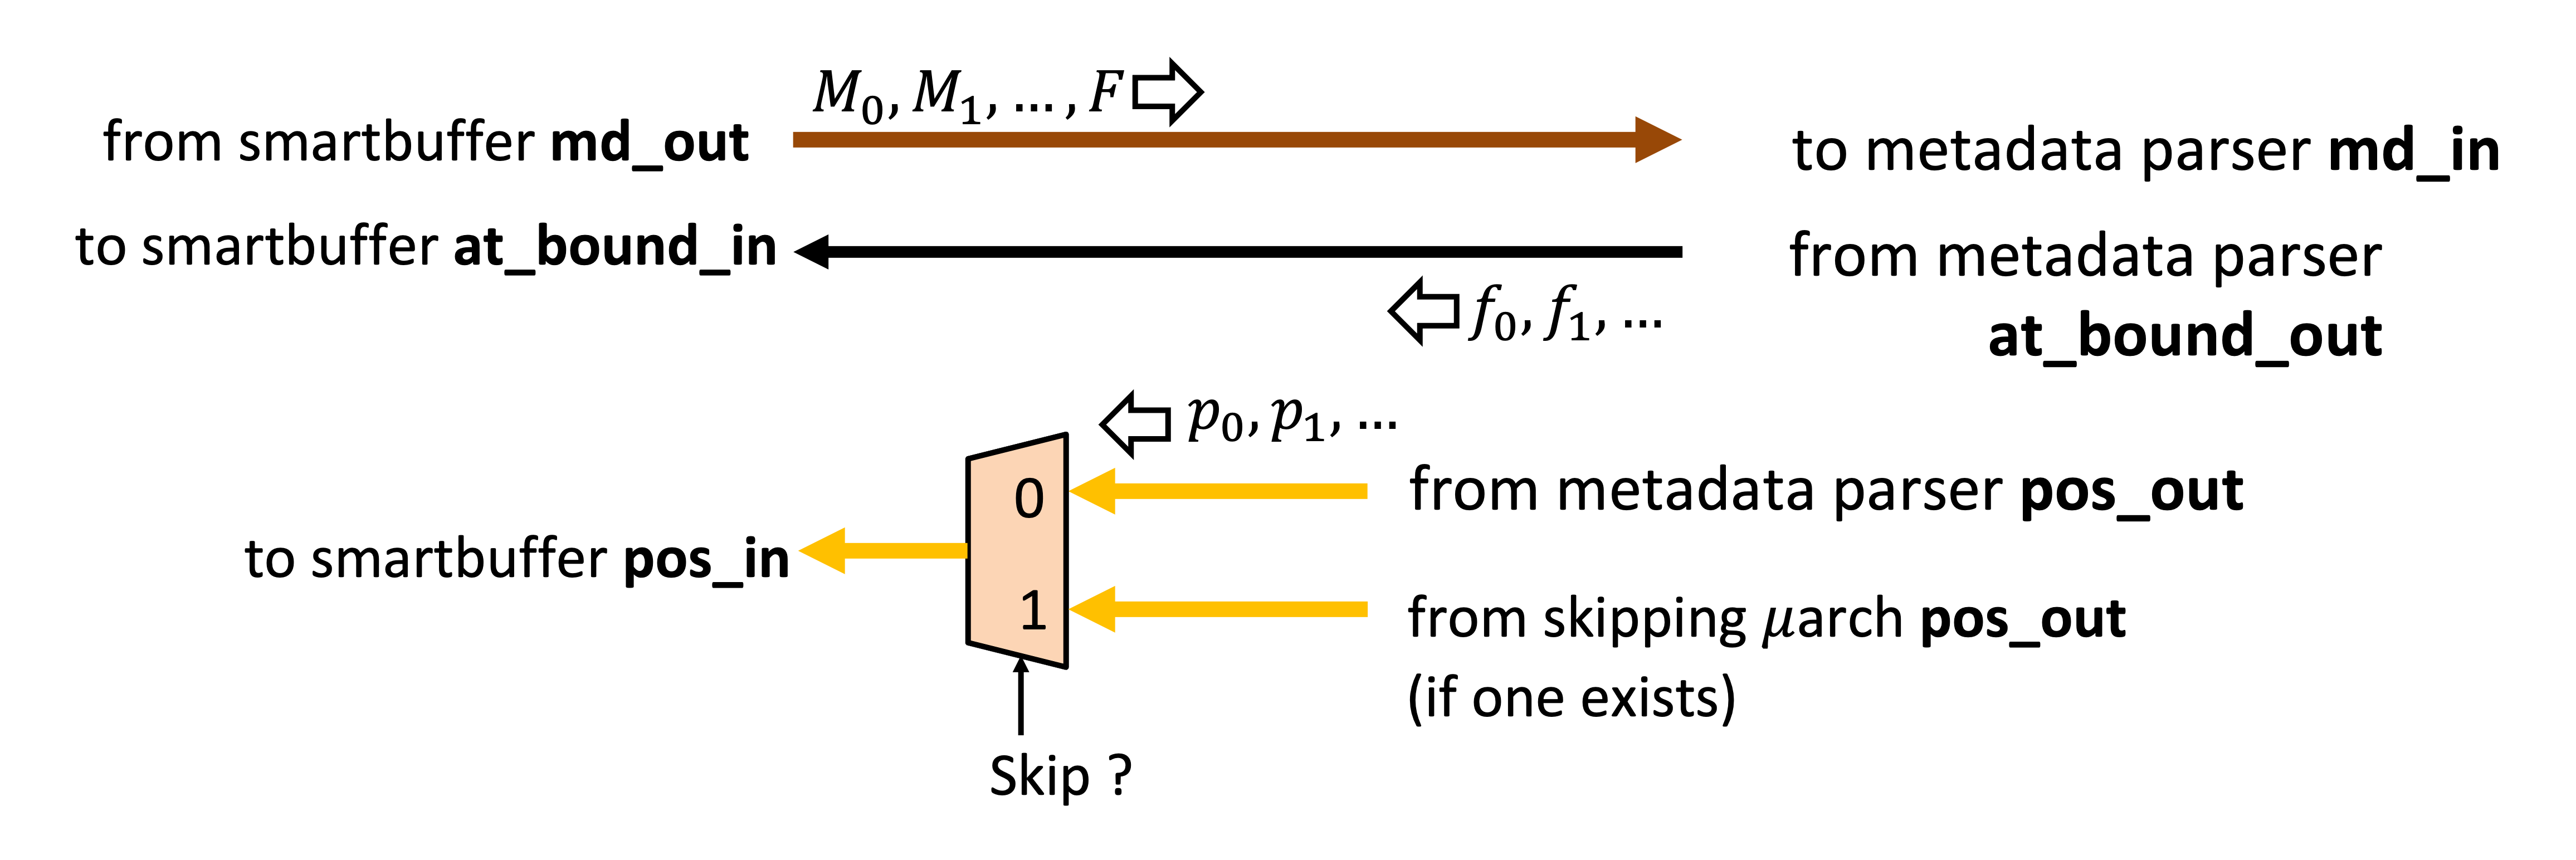
\includegraphics[width=0.95\textwidth]{figures/format_interface.png}
    \caption{Format interface I/O bundle. Sparse metadata moves from md\_out to md\_in. Payload lookup address offsets move from pos\_out to pos\_in. at\_bound\_out signals that fiber traversal is complete. The MUX that switches pos\_in between the metadata parser and the skipping microarchitecture is technically not part of the I/O bundle but is included for clarity and context.}
    \label{fig:format_interface}
\end{figure}